\chapter{BŞEÜ ÖĞRENCİ YARDIM MASASI ASİSTANI}
\label{ch:uygulama}

Bu bölümde geliştirilen uygulamanın mimarisi, kod yapısı, veri modeli, kullanıcı arayüzleri,
güvenlik önlemleri ve kalite süreci anlatılmaktadır. Sistem
\url{https://bseu-helpdesk.onrender.com} adresinde canlıdır; kaynak kodu
\url{https://github.com/AhmedElghazzawy/ai-ticket-assistant} adresindedir.

\section{Sistem Mimarisi ve Dağıtım}

Sistem tek bir Docker kapsayıcısında çalışan bir FastAPI uygulamasıdır: aynı uygulama hem JSON API'yi
sunar hem de derlenmiş React arayüzünü dağıtır. Veriler barındırılan bir PostgreSQL veritabanında,
vektörlerle birlikte tutulur (Şekil~\ref{fig:dagitim}). Tek bir dağıtım birimi bilinçli bir
seçimdir: tek kişilik bir projede ayrı servisler bir kazanç sağlamaz, ücretsiz katman da tek bir
kapsayıcı çalıştırır.

\begin{figure}[!ht]
\centering
\begin{tikzpicture}[node distance=8mm and 12mm]
  \node[kutu, minimum width=30mm, minimum height=16mm, fill=acik] (spa) {\textbf{Tarayıcı}\\React 19 SPA\\\scriptsize sohbet · Taleplerim · personel};
  \node[kutu, right=16mm of spa, minimum width=36mm, minimum height=16mm, fill=s3!10, draw=s3!80!black] (api) {\textbf{FastAPI uygulaması}\\\scriptsize JSON API + derlenmiş arayüz\\\scriptsize Docker, Render (Frankfurt)};
  \node[dbkutu, right=16mm of api, minimum width=30mm, minimum height=18mm] (db) {\textbf{Neon PostgreSQL 18}\\\scriptsize + pgvector};
  \node[kutu, below=12mm of api, minimum width=36mm, fill=s1!10, draw=s1] (gem) {\textbf{Google Gemini API}\\\scriptsize sınıflandır · yaz · gömme};
  \node[kutu, above=10mm of api, minimum width=36mm, fill=white, dashed] (gh) {\textbf{GitHub Actions (CI)}\\\scriptsize testler geçmeden yayın yok};
  \draw[ok, <->] (spa) -- node[etiket, above] {HTTPS} node[etiket, below] {\tiny OpenAPI istemcisi} (api);
  \draw[ok, <->] (api) -- node[etiket, above] {psycopg 3} node[etiket, below] {\tiny TLS, havuz} (db);
  \draw[ok, <->] (api) -- node[etiket, right] {\scriptsize zaman aşımı + model zinciri} (gem);
  \draw[kesik] (gh) -- node[etiket, right] {\scriptsize dağıtım} (api);
\end{tikzpicture}
\caption{Dağıtım şeması: tek kapsayıcı, tek veritabanı}
\label{fig:dagitim}
\end{figure}

\section{Bir Talebin İşlenmesi}

Bir talep gönderildiğinde önce istek sınırı ve günlük üst sınır kontrol edilir; reddedilen istek hiçbir
model çağrısı yapmaz. Sınıflandırma ile belge arama ve cevap yazma birbirinden bağımsız olduğu için
\textbf{paralel} çalışır; öğrenci iki model çağrısının toplamını değil, yavaş olanını bekler
(Şekil~\ref{fig:sira}). Talep ve onun ``oluşturuldu'' geçmiş kaydı tek bir SQL cümlesiyle yazılır.

\begin{figure}[!ht]
\centering
\begin{tikzpicture}[x=1cm, y=-0.78cm, every node/.style={font=\scriptsize}]
  \foreach \x/\n in {0/Tarayıcı, 2.3/API, 4.6/Kullanım durumu, 6.9/Sınıflandırıcı, 9.2/Arama + Cevap, 11.5/Karar, 13.8/Postgres}{
    \node[kutu, minimum width=19mm, minimum height=6mm, font=\scriptsize\bfseries] at (\x,0) {\n};
    \draw[gray!60, dashed] (\x,0.6) -- (\x,13.2);
  }
  \draw[ok] (0,1.4) -- node[above] {POST /api/tickets} (2.3,1.4);
  \node[fill=acik, draw=gray!50, rounded corners=1pt, align=center] at (2.3,2.6) {doğrula, günlük sınır,\\istek sınırı};
  \draw[ok] (2.3,3.8) -- node[above] {submit\_ticket} (4.6,3.8);
  \fill[s1!6] (4.75,4.5) rectangle (10.4,8.4);
  \node[text=s1, anchor=west] at (4.8,4.9) {paralel};
  \draw[ok] (4.6,5.8) -- node[above] {classify (çitli talep)} (6.9,5.8);
  \draw[ok] (4.6,7.2) -- node[above] {embed, ilk 3, cevap} (9.2,7.2);
  \draw[ok, dashed] (6.9,8.0) -- node[below] {etiketler} (4.6,8.0);
  \draw[ok] (4.6,9.4) -- node[above] {decide(...)} (11.5,9.4);
  \draw[ok, dashed] (11.5,10.3) -- node[above] {auto\_send + nedenler} (4.6,10.3);
  \draw[ok] (4.6,11.4) -- node[above] {talep + ``created'' olayı (tek SQL)} (13.8,11.4);
  \draw[ok, dashed] (4.6,12.6) -- node[below] {öğrencinin göreceği cevap + erişim kodu (bir kez)} (0,12.6);
\end{tikzpicture}
\caption{Bir talebin sistemdeki sıralı akışı (sınıflandırma ve cevap adımı paralel)}
\label{fig:sira}
\end{figure}

\subsection{Dayanıklı Model Zinciri}

Ücretsiz katmandaki modeller sık sık meşgul (HTTP 429/503) olabilmekte veya bağlantıyı
koparabilmektedir. Canlı sistem bu nedenle üç farklı ücretsiz modelden oluşan bir zincir kullanır
(ADR~0018, Şekil~\ref{fig:zincir}): meşgul olan model işi hemen bir sonrakine devreder; yavaş olan
modele 9 saniye sonra ikinci model eşlik eder (\textit{hedged request} \cite{dean2013}) ve ilk gelen
cevap kazanır; hiçbir öğrenci 25 saniyeden fazla beklemez; hata veren model 120 saniye zincirin
sonuna alınır (\textit{circuit breaker}). Değerlendirmeler bu zinciri kullanmaz; bir skor yalnızca
tek bir modeli ölçer.

\begin{figure}[!ht]
\centering
\begin{tikzpicture}[x=0.52cm, y=1cm, every node/.style={font=\scriptsize}]
  \draw[->, thick, koyu] (0,0) -- (26.5,0) node[right] {sn};
  \foreach \t in {0,5,9,15,20,25} { \draw (\t,0.1) -- (\t,-0.1) node[below] {\t}; }
  \fill[s1!35, rounded corners=2pt] (0,0.45) rectangle (14,0.95);
  \node[anchor=west] at (0.2,0.7) {Model 1: \texttt{3.5-flash-lite} (yavaş)};
  \fill[s3!45, rounded corners=2pt] (9,1.15) rectangle (13,1.65);
  \node[anchor=west] at (9.1,1.4) {Model 2 \checkmark};
  \node[anchor=west] at (13.3,1.4) {ilk gelen cevap kazanır, diğeri iptal};
  \draw[bseu, very thick, dashed] (25,-0.1) -- (25,2.0) node[above] {üst sınır 25 sn};
  \draw[s2, thick, dashed] (9,-0.1) -- (9,2.0) node[above] {9 sn: hedge};
  \node[draw=s2, fill=s2!8, rounded corners=2pt, anchor=west, align=left] at (15.5,0.55)
      {429/503 veya kopan bağlantı:\\ hemen sonraki modele geç};
\end{tikzpicture}
\caption[Canlı model zinciri]{Canlı model zinciri (\texttt{3.5-flash-lite}, \texttt{4-hydrogen}, \texttt{3.1-flash-lite})}
\label{fig:zincir}
\end{figure}

\section{Kod Katmanları ve Klasör Yapısı}

Arka uç, kurulabilir bir Python paketidir (\texttt{src/helpdesk/}). Bir katman yalnızca altındaki
katmanları içe aktarabilir (Şekil~\ref{fig:katman}). \texttt{tests/test\_architecture.py} her içe
aktarmayı ayrıştırır ve kural bozulursa CI başarısız olur. SQL yalnızca \texttt{storage/} katmanında,
model çağrıları yalnızca \texttt{ai/} katmanında bulunur.

\begin{figure}[!ht]
\centering
\begin{tikzpicture}[node distance=4mm and 6mm, every node/.style={font=\small}]
  \node[kutu, minimum width=26mm, fill=acik] (core) {\textbf{core}\\\scriptsize ayarlar · yollar · loglar};
  \node[kutu, above=of core, minimum width=26mm, fill=s3!12, draw=s3!80!black] (domain) {\textbf{domain}\\\scriptsize saf kurallar ve veri};
  \node[kutu, above left=5mm and -2mm of domain, minimum width=26mm, fill=s1!10, draw=s1] (ai) {\textbf{ai}\\\scriptsize Gemini adımları};
  \node[kutu, above right=5mm and -2mm of domain, minimum width=26mm, fill=s2!10, draw=s2] (storage) {\textbf{storage}\\\scriptsize tüm SQL};
  \node[kutu, above=18mm of domain, minimum width=30mm] (retrieval) {\textbf{retrieval}\\\scriptsize gömme + pgvector};
  \node[kutu, above=of retrieval, minimum width=30mm] (services) {\textbf{services}\\\scriptsize kullanım durumları};
  \node[kutu, above left=5mm and -4mm of services, minimum width=26mm] (api) {\textbf{api}\\\scriptsize ince HTTP};
  \node[kutu, above right=5mm and -4mm of services, minimum width=26mm] (evals) {\textbf{evals}\\\scriptsize gerçek ölçümler};
  \foreach \a/\b in {domain/core, ai/domain, storage/domain, retrieval/ai, retrieval/storage, services/retrieval, api/services, evals/services}
    \draw[ok] (\a) -- (\b);
  \node[right=22mm of domain, align=left, font=\scriptsize, text width=46mm] {Ok yönü: ``içe aktarabilir''.\\ Yukarı doğru bir içe aktarma\\ \texttt{test\_architecture.py} tarafından\\ reddedilir.};
\end{tikzpicture}
\caption{Kod katmanları ve izin verilen bağımlılık yönü}
\label{fig:katman}
\end{figure}

Projenin klasör yapısı Şekil~\ref{fig:klasor}'da gösterilmiştir.

\begin{figure}[!ht]
\centering
\begin{minipage}{0.92\textwidth}
\footnotesize\singlespacing
\renewcommand*\DTstylecomment{\rmfamily\color{gray!70!black}\itshape}
\renewcommand*\DTstyle{\ttfamily}
\setlength{\DTbaselineskip}{11.2pt}
\dirtree{%
.1 ai-ticket-assistant/.
.2 src/helpdesk/\DTcomment{arka uç paketi (Python 3.12)}.
.3 core/\DTcomment{tipli ayarlar (ortamı okuyan tek modül), loglar}.
.3 domain/\DTcomment{decision.py, grounding.py, offices.py, outputs.py, records.py}.
.3 ai/\DTcomment{classifier.py, answer.py, fence.py, gemini.py, resilience.py}.
.3 storage/\DTcomment{db.py (yalnızca eklenen migration'lar), tickets.py, staff.py}.
.3 retrieval/\DTcomment{knowledge\_base.py, embeddings.py, search.py}.
.3 services/\DTcomment{pipeline, student\_tickets, staff\_desk, auth, insights}.
.3 api/\DTcomment{app.py (bileşim kökü), routers/, security.py}.
.3 evals/\DTcomment{classifier, retrieval, pipeline, security, stats (Wilson)}.
.2 frontend/\DTcomment{React 19 + TypeScript, üretilmiş API istemcisi, e2e/ (Playwright)}.
.2 tests/\DTcomment{316 pytest testi, gerçek Postgres, sahte model (fakes.py)}.
.2 data/.
.3 knowledge\_base/\DTcomment{28 resmî belge (14 konu × TR/EN)}.
.3 tickets/\DTcomment{tickets.jsonl (dev 80), test\_tickets, realistic\_tickets (kilitli)}.
.3 kb\_index.json\DTcomment{190 parça ve 768 boyutlu vektörleri}.
.2 eval/\DTcomment{sürümlü değerlendirme sonuçları (JSON)}.
.2 docs/\DTcomment{labels.md, PROJECT\_BRIEF.md, ROADMAP.md, decisions/ (18 ADR)}.
.2 Dockerfile, compose.yaml, render.yaml\DTcomment{kurulum ve dağıtım}.
.2 .github/workflows/\DTcomment{ci.yml, codeql.yml}.
.2 ARCHITECTURE.md, README.md, README.tr.md, Makefile.
}
\end{minipage}
\caption{Proje deposunun klasör yapısı}
\label{fig:klasor}
\end{figure}

\section{Veri Modeli ve Talep Yaşam Döngüsü}

Veritabanında altı tablo bulunur (Şekil~\ref{fig:er}). \texttt{tickets} tablosu talebi, etiketleri,
taslağı ve kararı tutar. \texttt{ticket\_events} tablosu yalnızca ekleme yapılabilen bir geçmiş
kaydıdır: bir veritabanı tetikleyicisi (trigger) her \texttt{UPDATE} işlemini reddeder ve talepteki
her değişiklik, kaydıyla birlikte aynı SQL cümlesinde yazılır (ADR~0017). Şema değişiklikleri
numaralı ve yalnızca eklenen migration adımlarıyla yapılır; ara rapor tarihinde şema sürümü 6'dır.

\begin{figure}[!ht]
\centering
\begin{tikzpicture}[every node/.style={font=\scriptsize}, tablo/.style={draw=koyu!70, rounded corners=2pt, fill=white, align=left, inner sep=3pt, anchor=north}]
  \node[tablo] (t) at (0,0) {\textbf{\normalsize tickets}\\[-4pt]\rule{3.4cm}{0.4pt}\\
    \underline{id} bigint\\ created\_at, language\\ text \textit{(kişisel veri)}\\ category, priority, escalate\\ ai\_reason, office\\ auto\_send, reasons (jsonb)\\ top\_score, draft, covered\\ sources (jsonb), general\_help\\ status, final\_reply\\ access\_hash \textit{(SHA-256)}\\ feedback, demo};
  \node[tablo] (e) at (5.2,0) {\textbf{\normalsize ticket\_events}\\[-4pt]\rule{3.4cm}{0.4pt}\\
    \underline{id} bigint\\ ticket\_id $\rightarrow$ tickets\\ at\\ kind: created | human\_requested\\ \quad | replied | reassigned\\ staff\_id $\rightarrow$ staff\\ detail (jsonb)\\[2pt] \textit{UPDATE yasak (trigger)}};
  \node[tablo] (s) at (10.2,0) {\textbf{\normalsize staff}\\[-4pt]\rule{3.4cm}{0.4pt}\\
    \underline{id} bigint\\ email (benzersiz)\\ name, role, office\\ password\_hash \textit{(Argon2id)}\\ demo};
  \node[tablo] (se) at (10.2,-3.4) {\textbf{\normalsize sessions}\\[-4pt]\rule{3.4cm}{0.4pt}\\
    \underline{token\_hash}\\ staff\_id $\rightarrow$ staff\\ expires\_at};
  \node[tablo] (kb) at (5.2,-4.0) {\textbf{\normalsize kb\_chunks}\\[-4pt]\rule{3.4cm}{0.4pt}\\
    \underline{id} (ör. sinavlar.tr\#3)\\ doc, language, title\\ source, url, text\\ embedding \textbf{vector(768)}};
  \node[tablo] (f) at (0,-5.2) {\textbf{\normalsize failed\_logins}\\[-4pt]\rule{2.4cm}{0.4pt}\\ key, at};
  \draw[ok] (e.west |- 0,-0.9) -- node[etiket, above] {1 : n} (t.east |- 0,-0.9);
  \draw[ok] (e.east |- 0,-1.6) -- node[etiket, above] {n : 1} (s.west |- 0,-1.6);
  \draw[ok] (se.north) -- (s.south);
\end{tikzpicture}
\caption{Veri modeli (şema sürümü 6)}
\label{fig:er}
\end{figure}

Bir talebin durumu Şekil~\ref{fig:yasam}'daki geçişlerle değişir. \texttt{auto\_send} sistemin
verdiği kararı, \texttt{status} ise talebin şu anki yerini kaydeder; bu ayrım, öğrenci otomatik
cevaptan sonra bir insana başvurduğunda bile kararın değerlendirmesini dürüst tutar.

\begin{figure}[!ht]
\centering
\begin{tikzpicture}[node distance=10mm and 26mm, durum/.style={draw=koyu!80, rounded rectangle, minimum width=26mm, minimum height=9mm, font=\small}]
  \node[circle, fill=koyu, inner sep=3pt] (b) {};
  \node[durum, right=16mm of b, yshift=12mm, fill=s3!12] (a) {\texttt{auto\_sent}};
  \node[durum, right=16mm of b, yshift=-12mm, fill=s2!12] (o) {\texttt{open}};
  \node[durum, right=of o, fill=s1!12] (h) {\texttt{handled}};
  \node[circle, draw=koyu, inner sep=1pt, right=14mm of h] (e) {\tikz\fill[koyu] circle (2.5pt);};
  \draw[ok] (b) -- node[etiket, above, sloped] {7 kontrol geçti} (a);
  \draw[ok] (b) -- node[etiket, below, sloped] {bir kontrol kaldı} (o);
  \draw[ok] (a) -- node[etiket, right, align=left] {öğrenci ``bir uzmana\\ gönder'' dedi} (o);
  \draw[ok] (o) to[loop below, looseness=5] node[etiket, below] {başka birime aktar} (o);
  \draw[ok] (o) -- node[etiket, above] {personel cevapladı} node[etiket, below] {\tiny (yalnızca biri kazanır)} (h);
  \draw[ok] (h) -- (e);
  \draw[ok] (a) -| (e);
\end{tikzpicture}
\caption{Talep yaşam döngüsü; her geçiş \texttt{ticket\_events} tablosuna da yazılır}
\label{fig:yasam}
\end{figure}

\section{Kullanıcı Arayüzleri}

Arayüz React 19 ile yazılmış, Türkçe ve İngilizce, açık ve koyu tema destekleyen, telefona uyumlu
tek sayfalı bir uygulamadır. Renkler BŞEÜ web sitesinin stil dosyasından alınmış ve kontrast
oranları denetlenmiştir; üniversitenin resmî logosu izin alınmadan kullanılmamıştır. Bu bölümdeki
ekran görüntüleri uygulamanın kendisinden alınmıştır: öğrenci ekranları canlı sistemde gerçek model
cevaplarıyla, personel ekranları ise demo modunda (gerçek boru hattı çıktısından üretilmiş örnek
taleplerle) yerel olarak çalıştırılan uygulamadan.

\subsection{Öğrenci Ekranları}

Öğrenci hesap açmadan sorusunu yazar (Şekil~\ref{fig:ogrenciana}). Ana sayfa, sistemin ölçülen
sonuçlarını ve bir örnek sorunun adım adım nasıl işlendiğini de gösterir.

\begin{figure}[!ht]
\centering
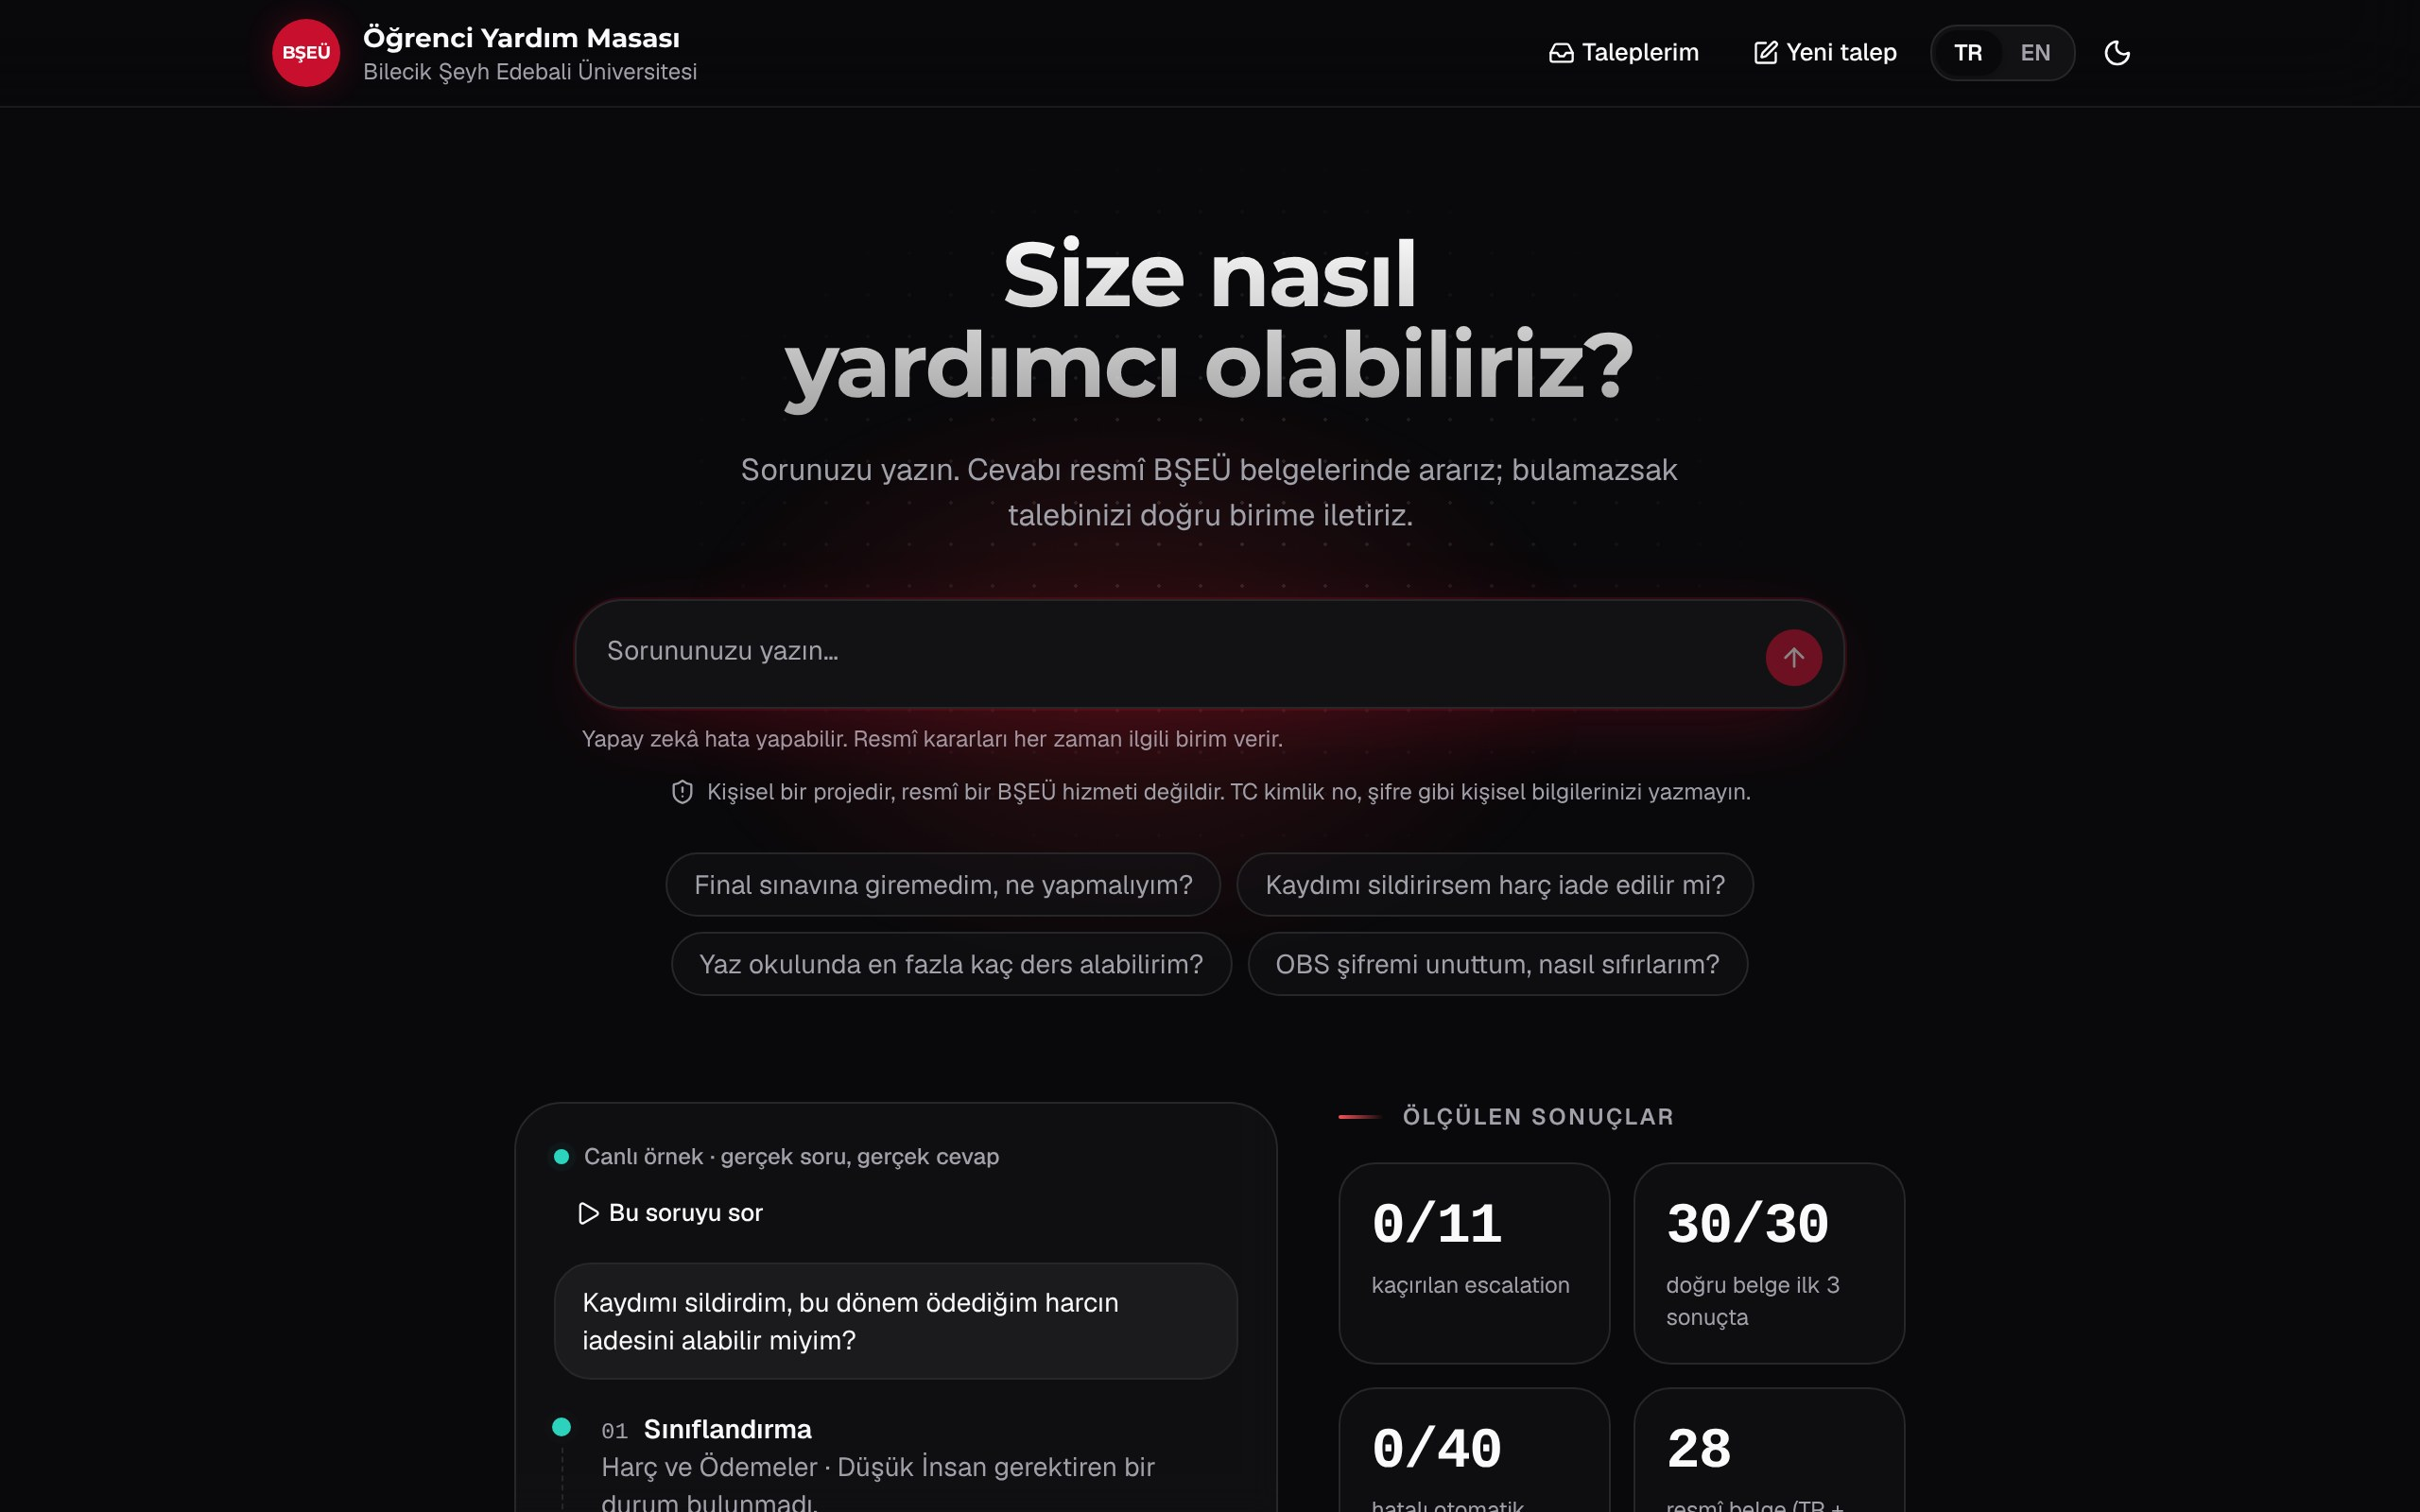
\includegraphics[width=0.95\textwidth]{sekiller/ogrenci_ana_sayfa.jpg}
\caption{Öğrenci ana sayfası: soru kutusu, örnek sorular ve resmî hizmet olmadığı uyarısı}
\label{fig:ogrenciana}
\end{figure}

Belgeler soruyu cevaplıyor ve yedi kontrolün hepsi geçiyorsa cevap hemen gösterilir
(Şekil~\ref{fig:otomatik}). Kaynak kartlarını model değil kod oluşturur; kart resmî sayfaya bağlanır.

\begin{figure}[!ht]
\centering
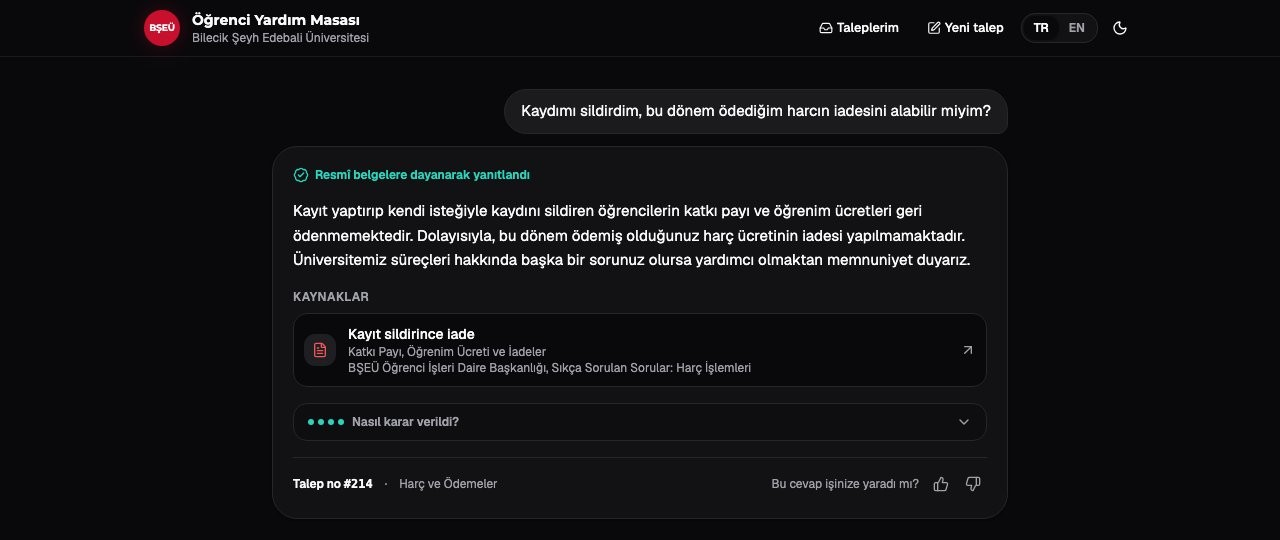
\includegraphics[width=0.95\textwidth]{sekiller/ogrenci_otomatik_cevap.jpg}
\caption{Otomatik cevap: ``Resmî belgelere dayanarak yanıtlandı'', kaynak kartı ve geri bildirim}
\label{fig:otomatik}
\end{figure}

Bir kontrol kaldığında talep birime iletilir. Escalation yoksa ve taslağın kaynaklı kısmı
doğrulandıysa bu kısım ``ön bilgi'' olarak hemen gösterilir. ``Nasıl karar verildi?'' paneli,
kararın arkasındaki gerçek kontrolleri adım adım açıklar (Şekil~\ref{fig:iz}).

\begin{figure}[!ht]
\centering
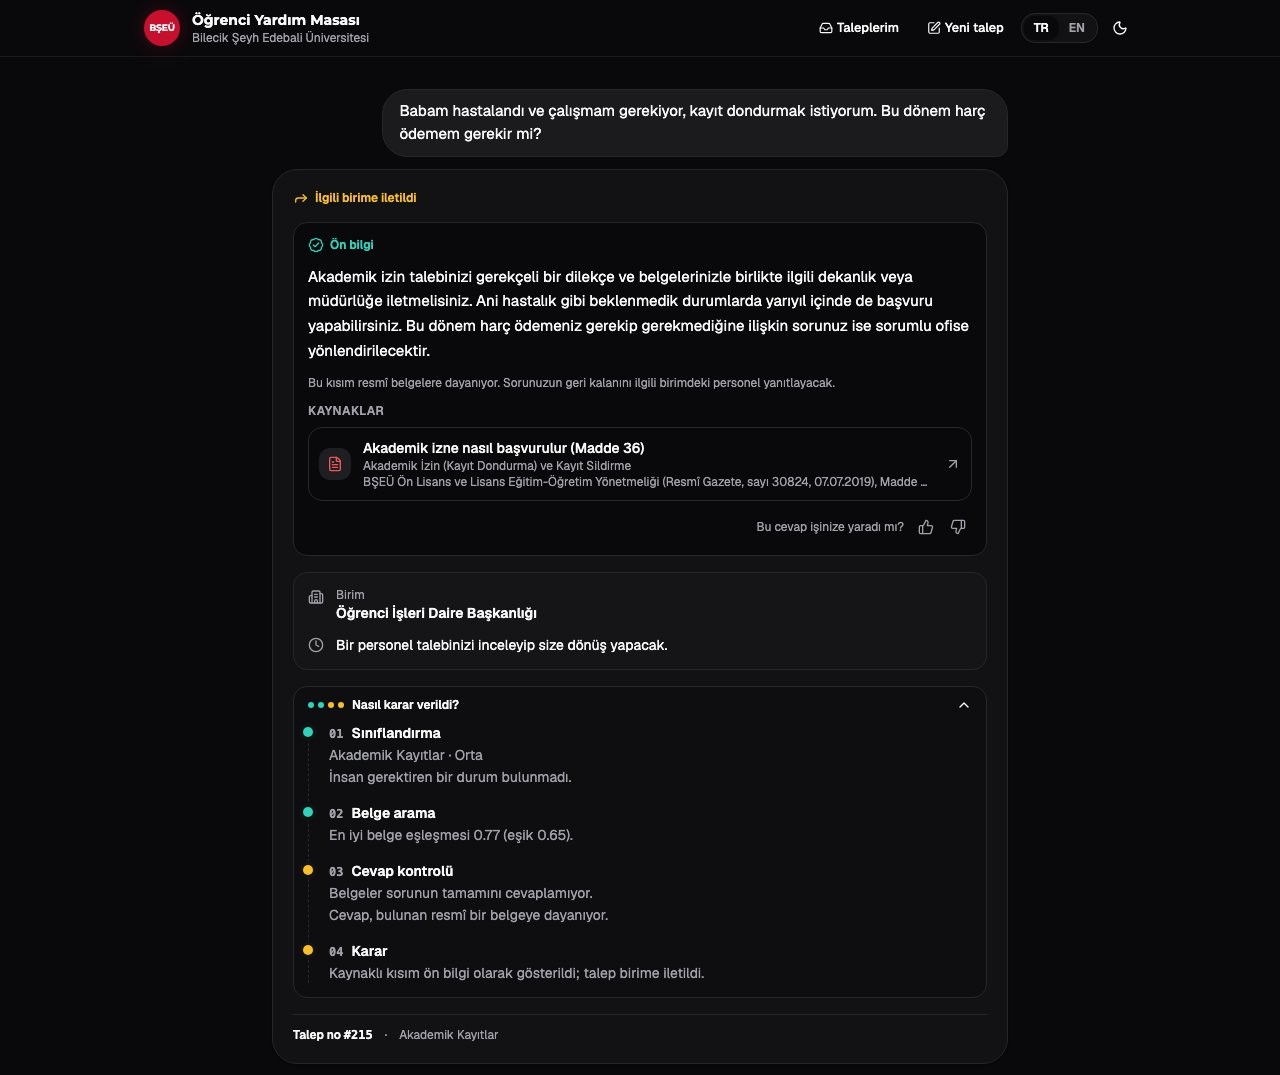
\includegraphics[width=0.82\textwidth]{sekiller/ogrenci_karar_izi.jpg}
\caption{Birime iletilen talep: ön bilgi, sorumlu birim ve ``Nasıl karar verildi?'' izi}
\label{fig:iz}
\end{figure}

Arayüz telefon ekranlarına da uyumludur (Şekil~\ref{fig:mobil}). Öğrenci her talep için bir kez
gösterilen gizli bir erişim koduyla ``Taleplerim'' sayfasından talebini takip edebilir, personelin
cevabını okuyabilir ve otomatik cevap işine yaramadıysa tek tıkla talebini bir uzmana gönderebilir.

\begin{figure}[!ht]
\centering
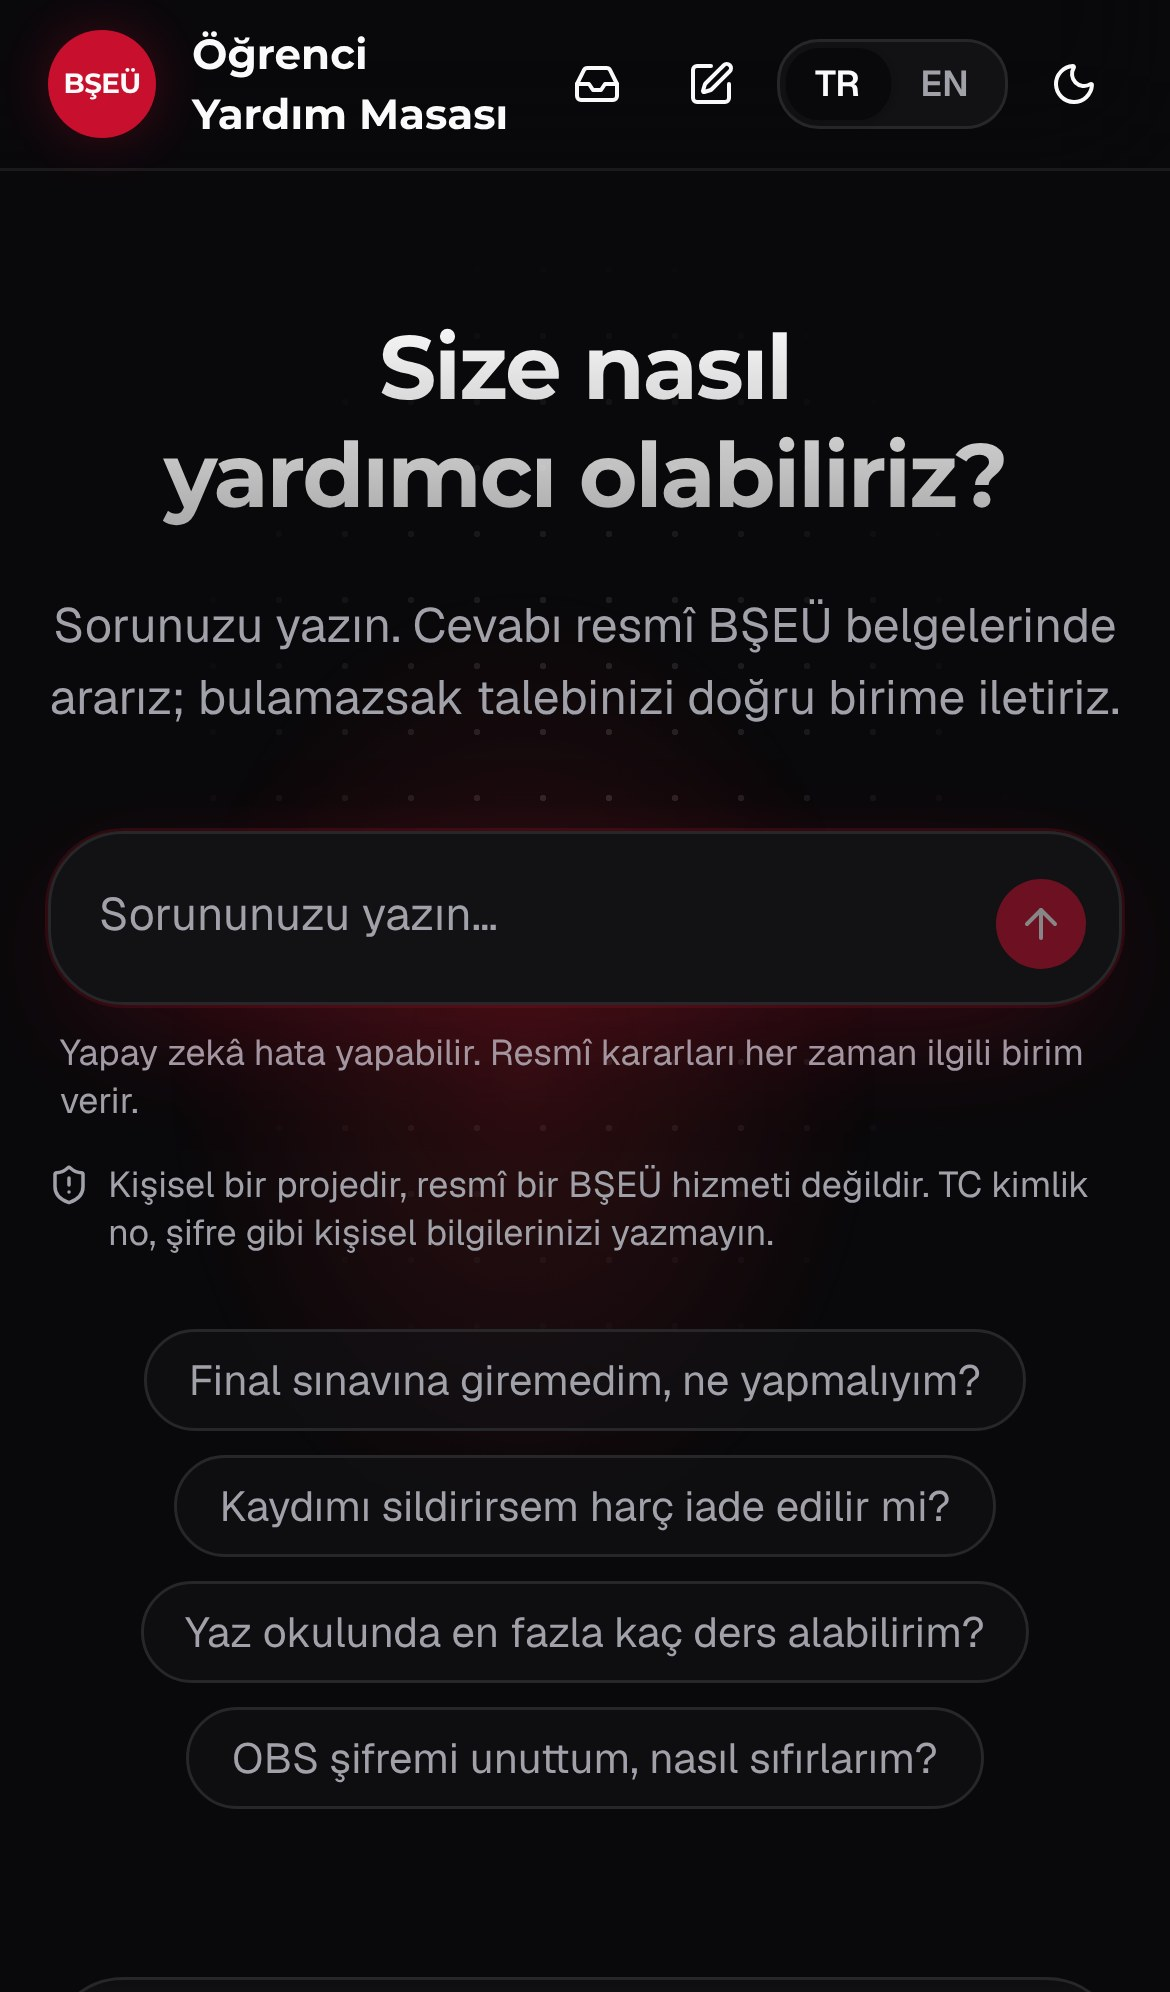
\includegraphics[width=0.36\textwidth]{sekiller/ogrenci_mobil.jpg}
\caption{Öğrenci sayfasının telefon görünümü}
\label{fig:mobil}
\end{figure}

\subsection{Personel Paneli}

Personel e-posta ve şifreyle giriş yapar; herkese açık kayıt yoktur. Demo modunda ``Demo olarak
dene'' düğmesi, yalnızca örnek talepleri gören bir demo hesabı açar (Şekil~\ref{fig:giris}).

\begin{figure}[!ht]
\centering
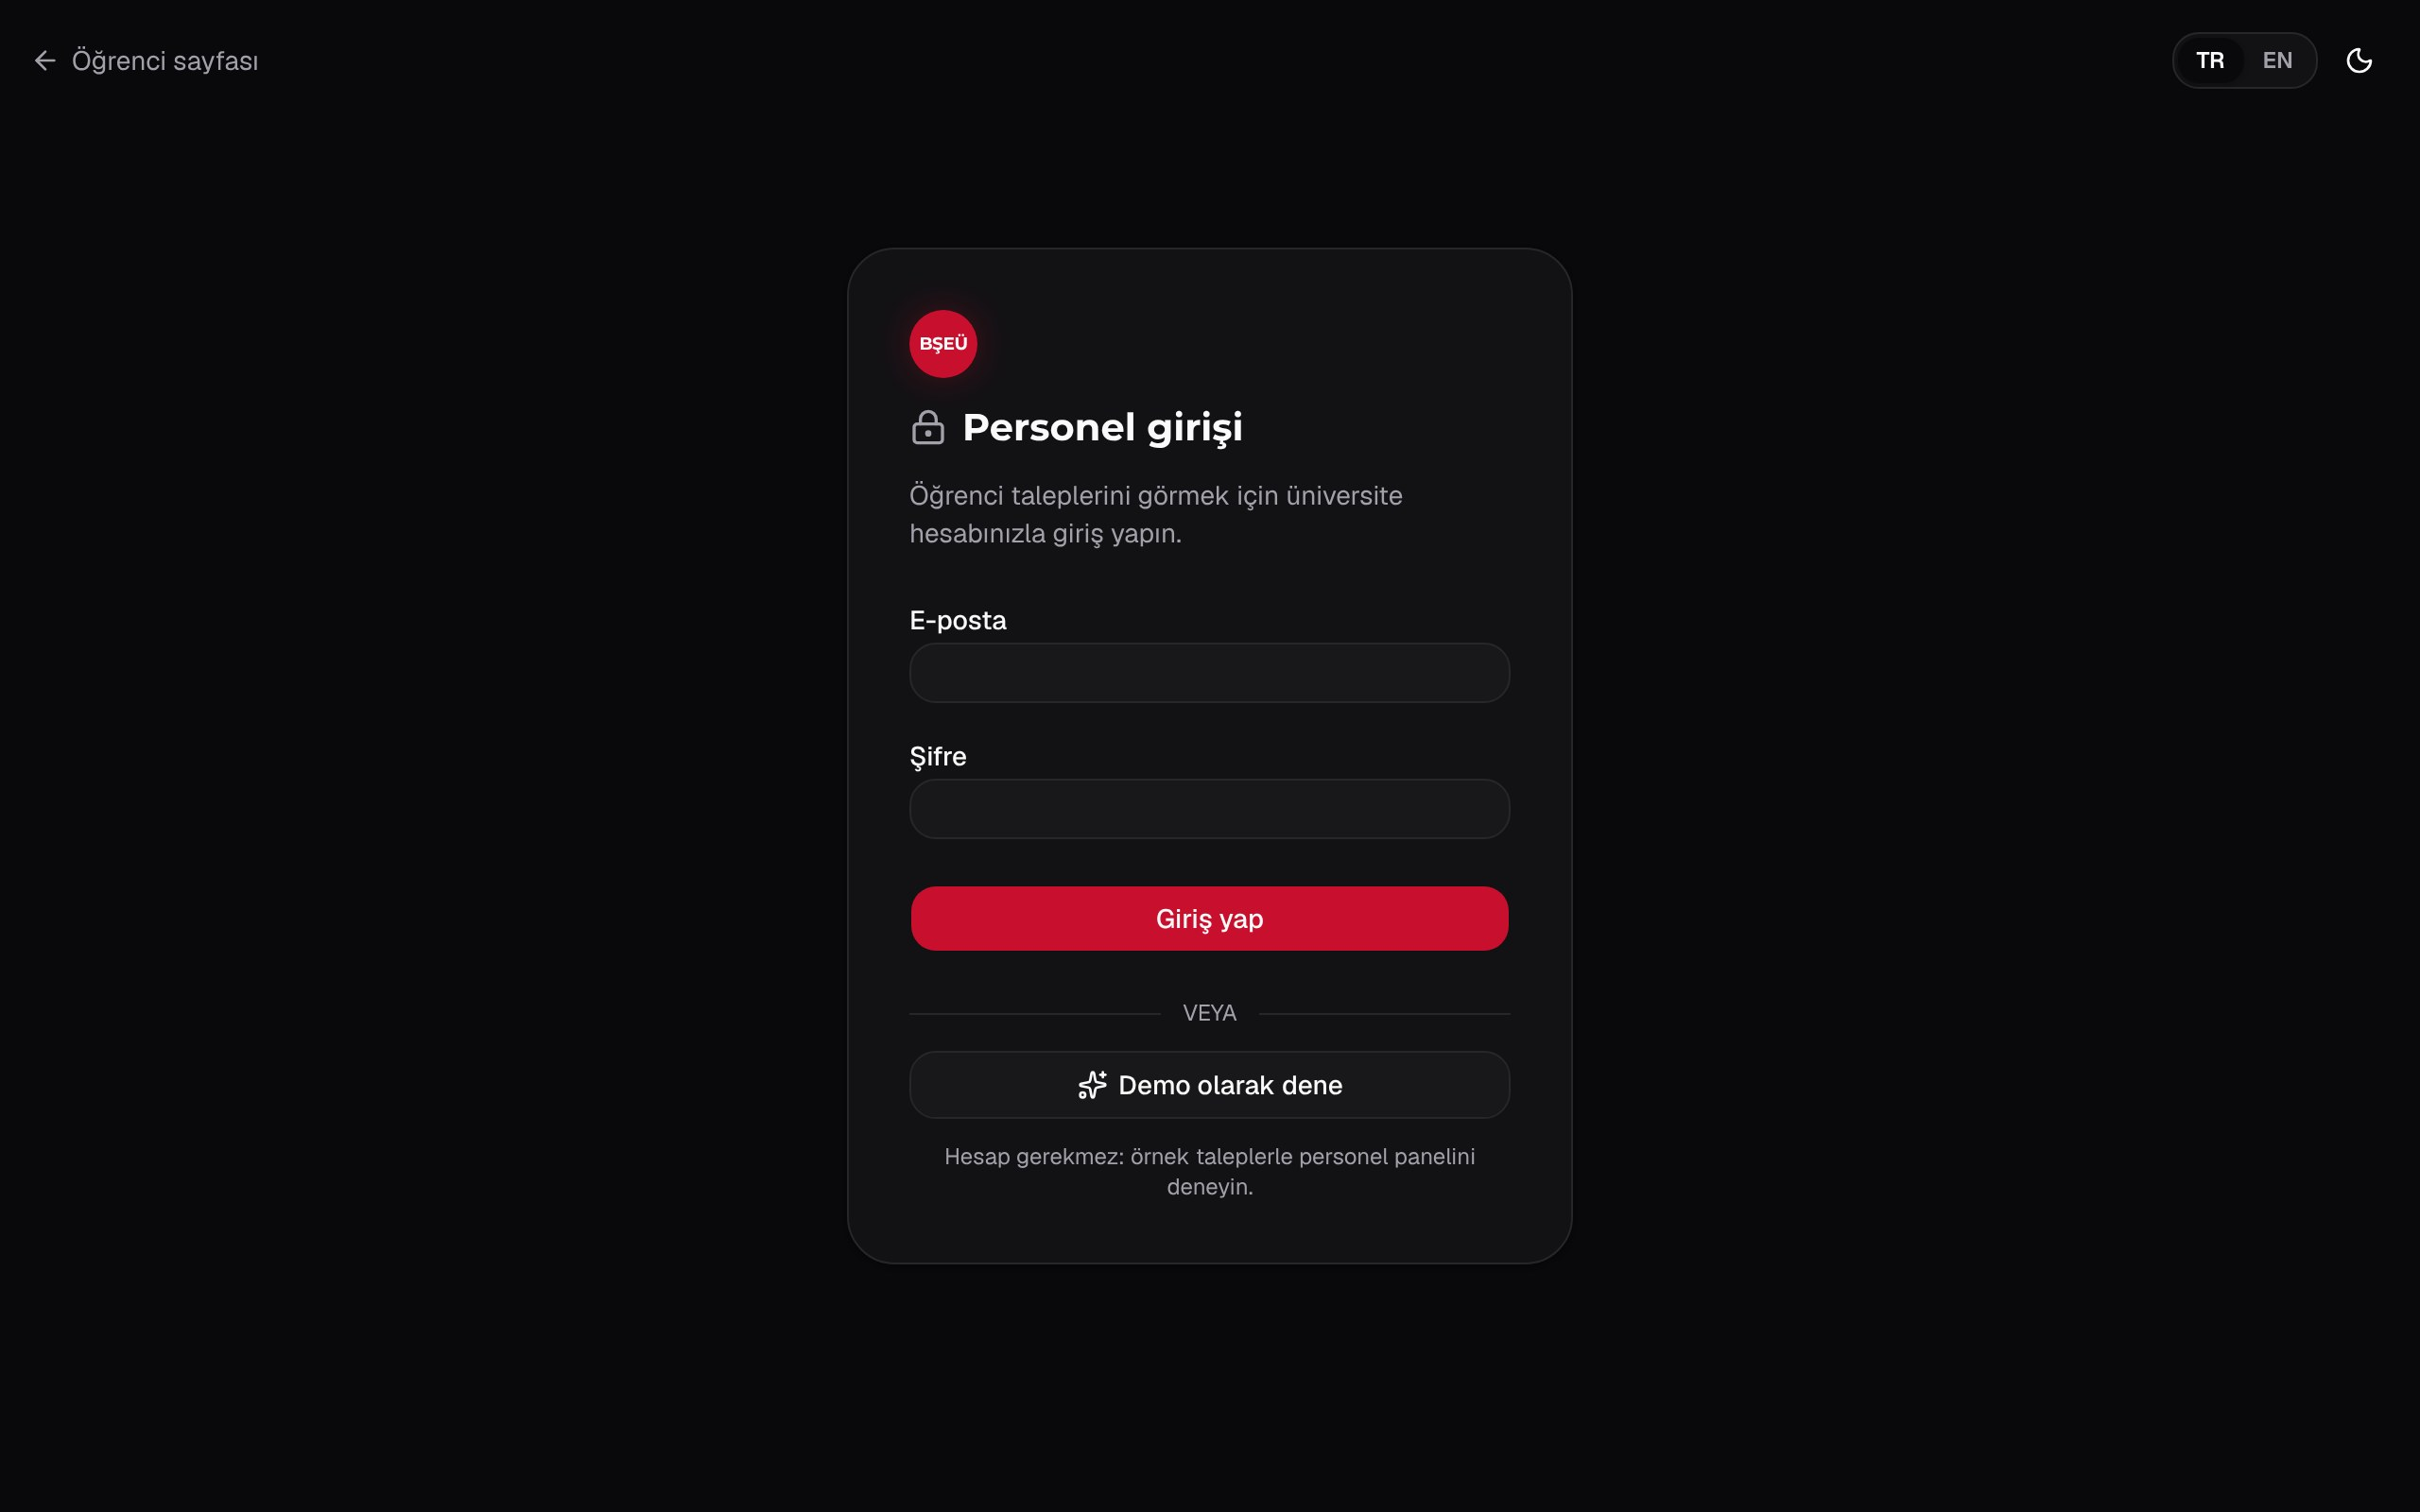
\includegraphics[width=0.7\textwidth]{sekiller/personel_giris.jpg}
\caption{Personel girişi ve demo düğmesi}
\label{fig:giris}
\end{figure}

İnceleme kuyruğu önce acil talepleri, sonra en uzun bekleyenleri gösterir
(Şekil~\ref{fig:kuyruk}). Personel yalnızca kendi biriminin taleplerini görür; başka birimin talebi,
var olmayan bir talep gibi 404 döner.

\begin{figure}[!ht]
\centering
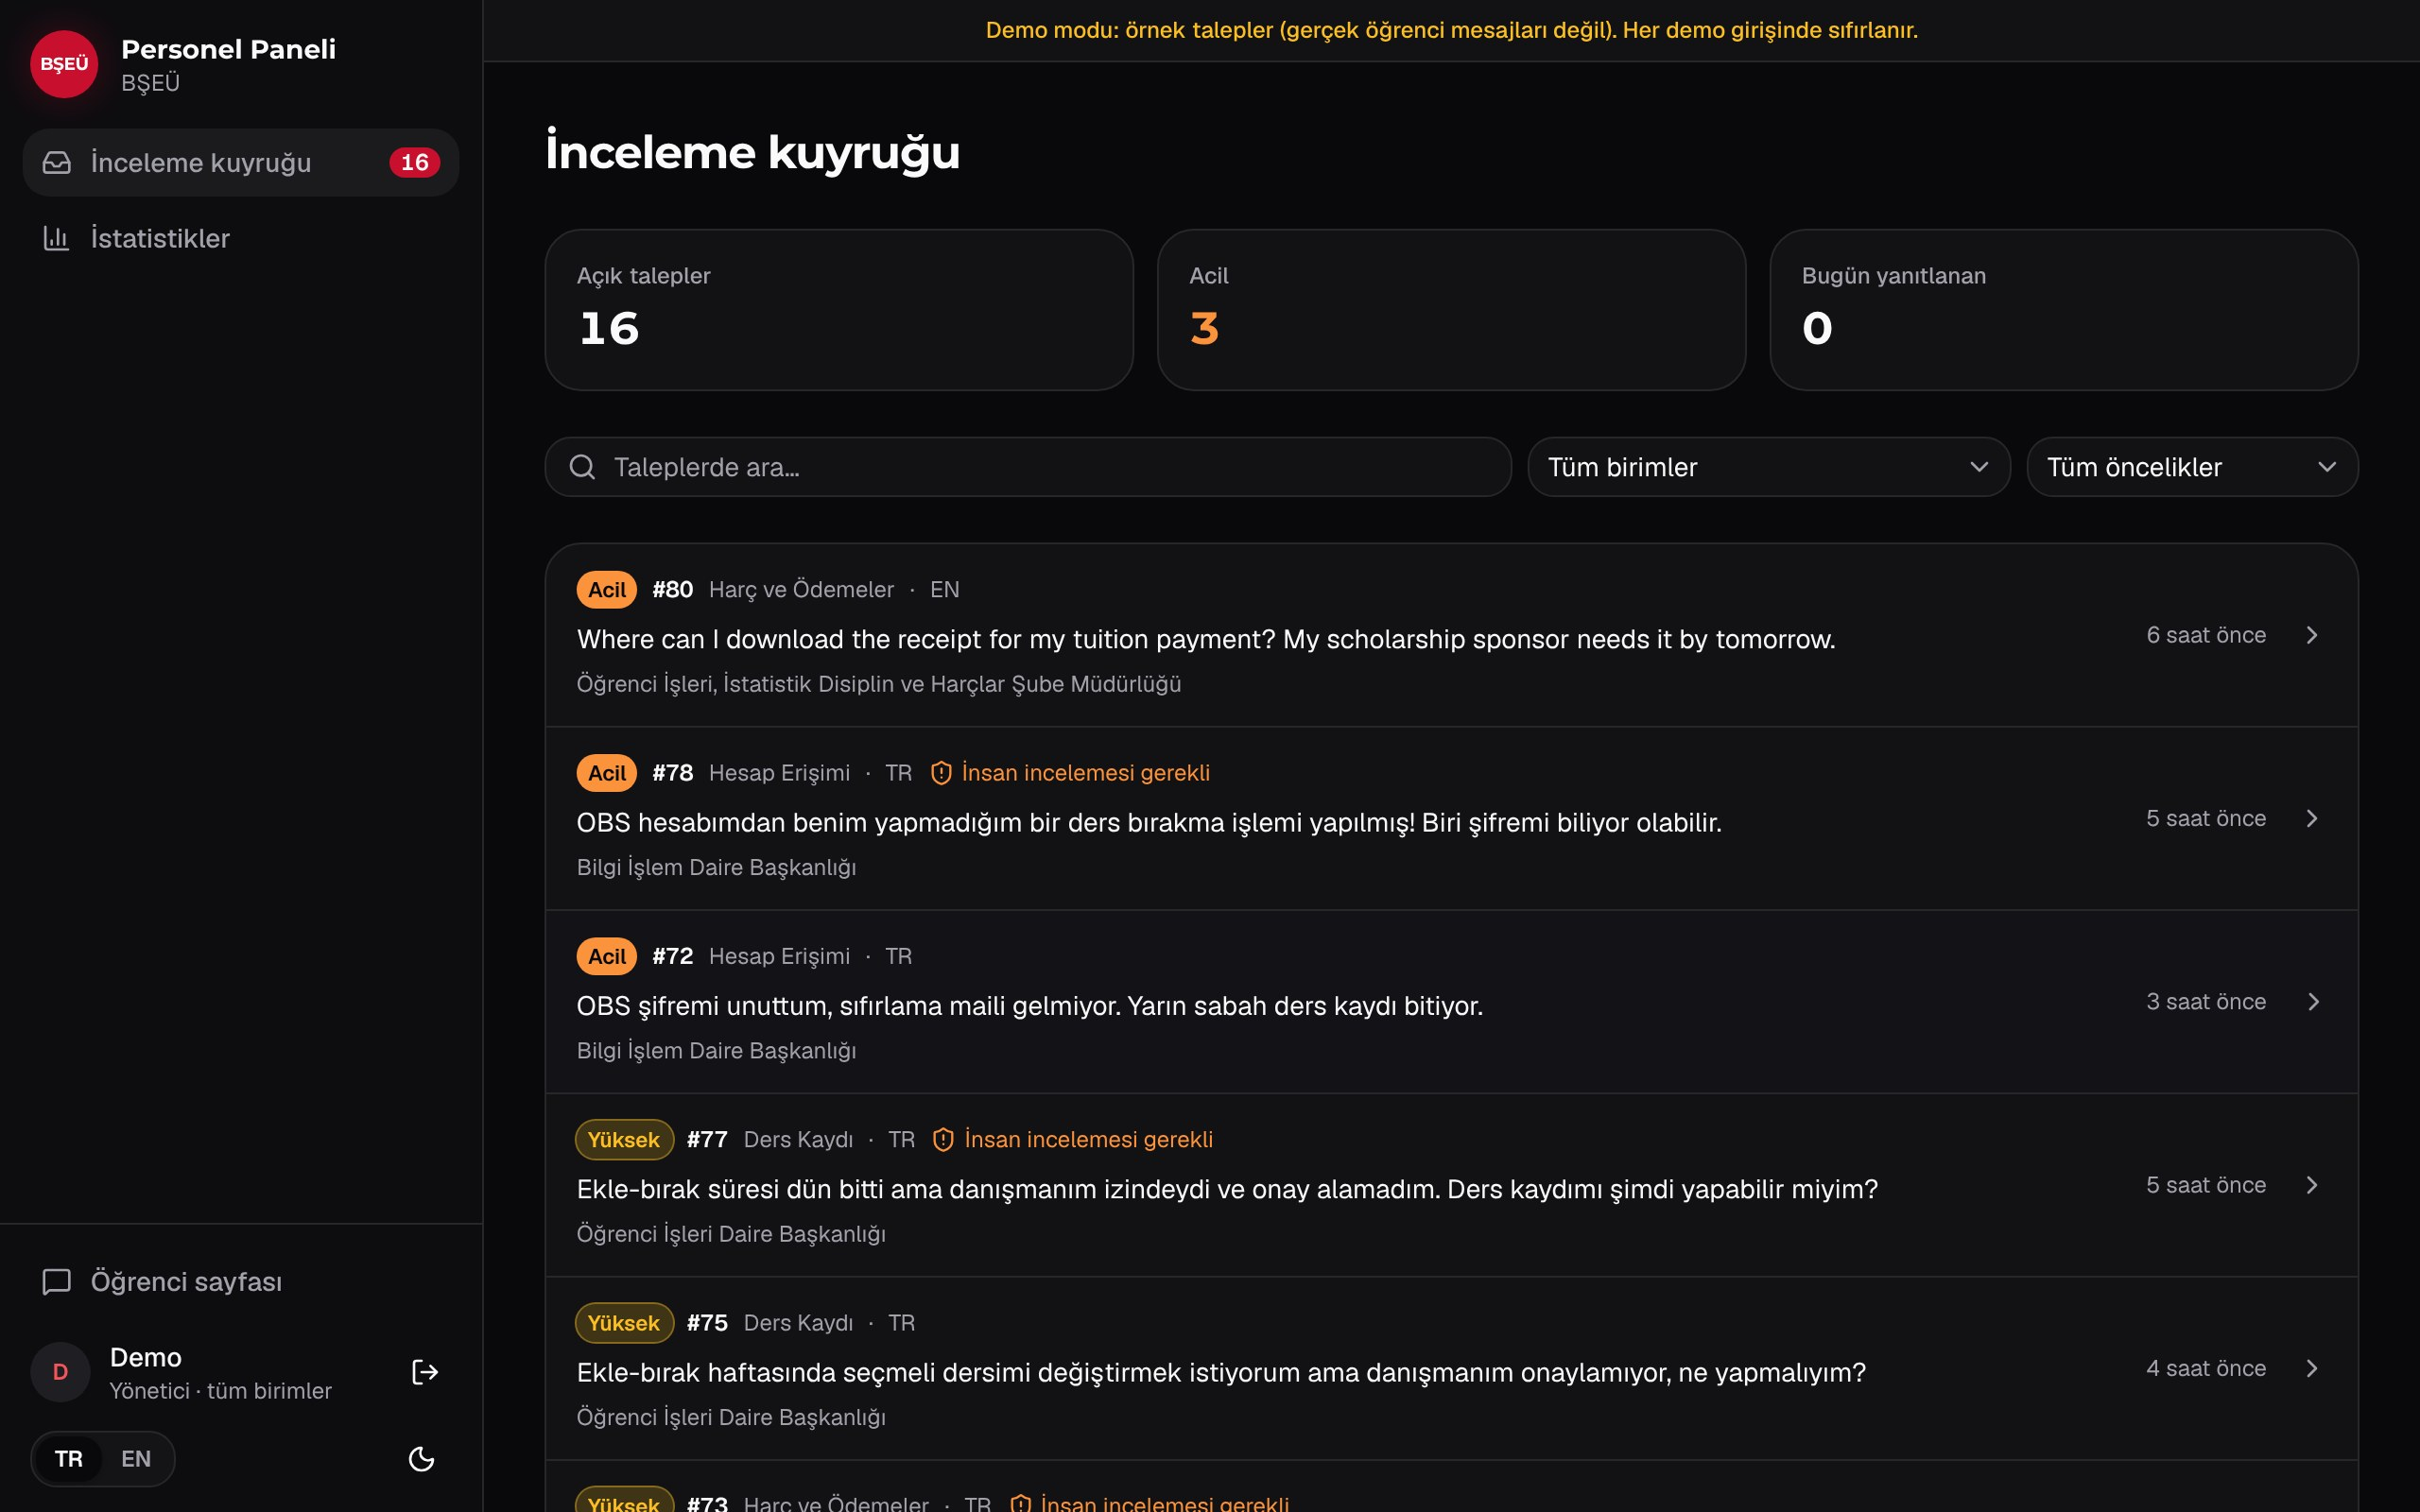
\includegraphics[width=0.95\textwidth]{sekiller/personel_kuyruk.jpg}
\caption{Personel inceleme kuyruğu (demo modu)}
\label{fig:kuyruk}
\end{figure}

Talep detayında öğrencinin mesajı, otomatik gönderilmeme nedenleri, modelin kendi gerekçesi,
kaynaklı ve düzenlenebilir taslak, taslağın kullandığı kaynaklar ve değiştirilemeyen geçmiş birlikte
görünür (Şekil~\ref{fig:detay}). Personel taslağı düzenleyip gönderebilir veya talebi başka bir
birime aktarabilir; iki personel aynı anda cevap verirse yalnızca biri kazanır.

\begin{figure}[!ht]
\centering
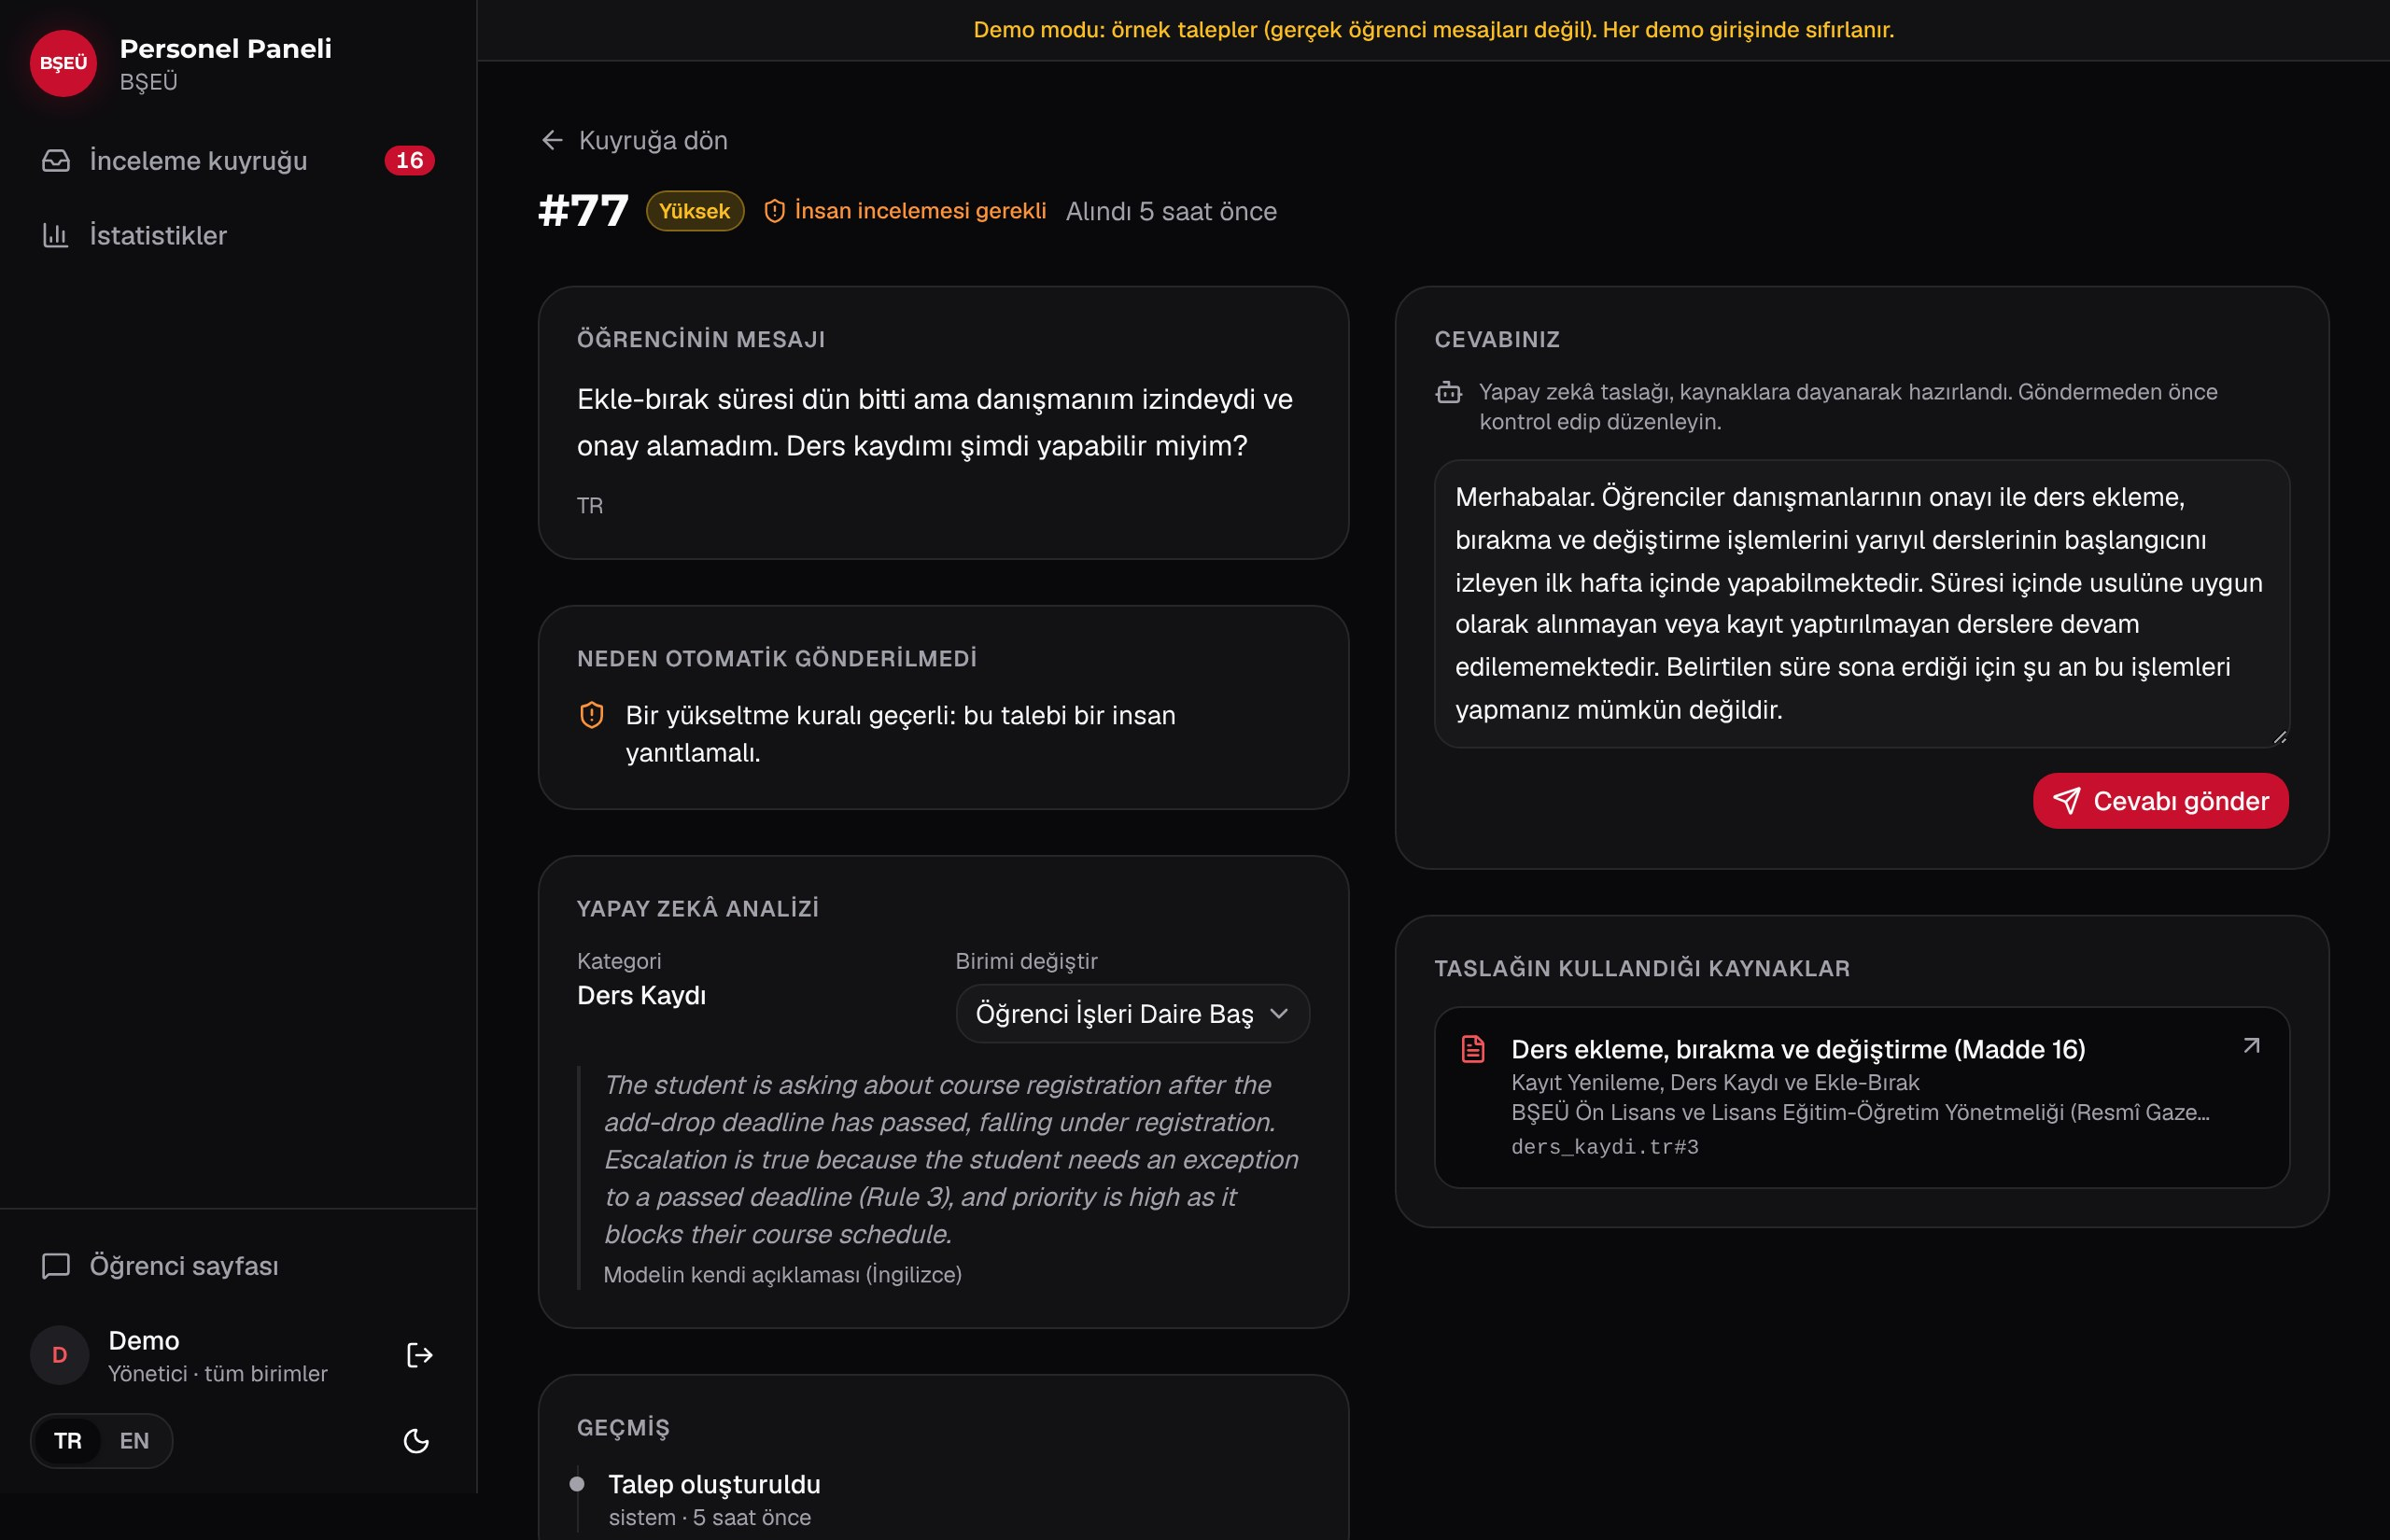
\includegraphics[width=0.95\textwidth]{sekiller/personel_talep_detay.jpg}
\caption{Talep detayı: nedenler, yapay zekâ analizi, kaynaklı taslak ve geçmiş}
\label{fig:detay}
\end{figure}

İstatistik sayfası taleplerin nasıl sonuçlandığını, kategorilere dağılımını ve son 14 günü gösterir
(Şekil~\ref{fig:istatistik}). Her kartta örnek sayısı da yazar.

\begin{figure}[!ht]
\centering
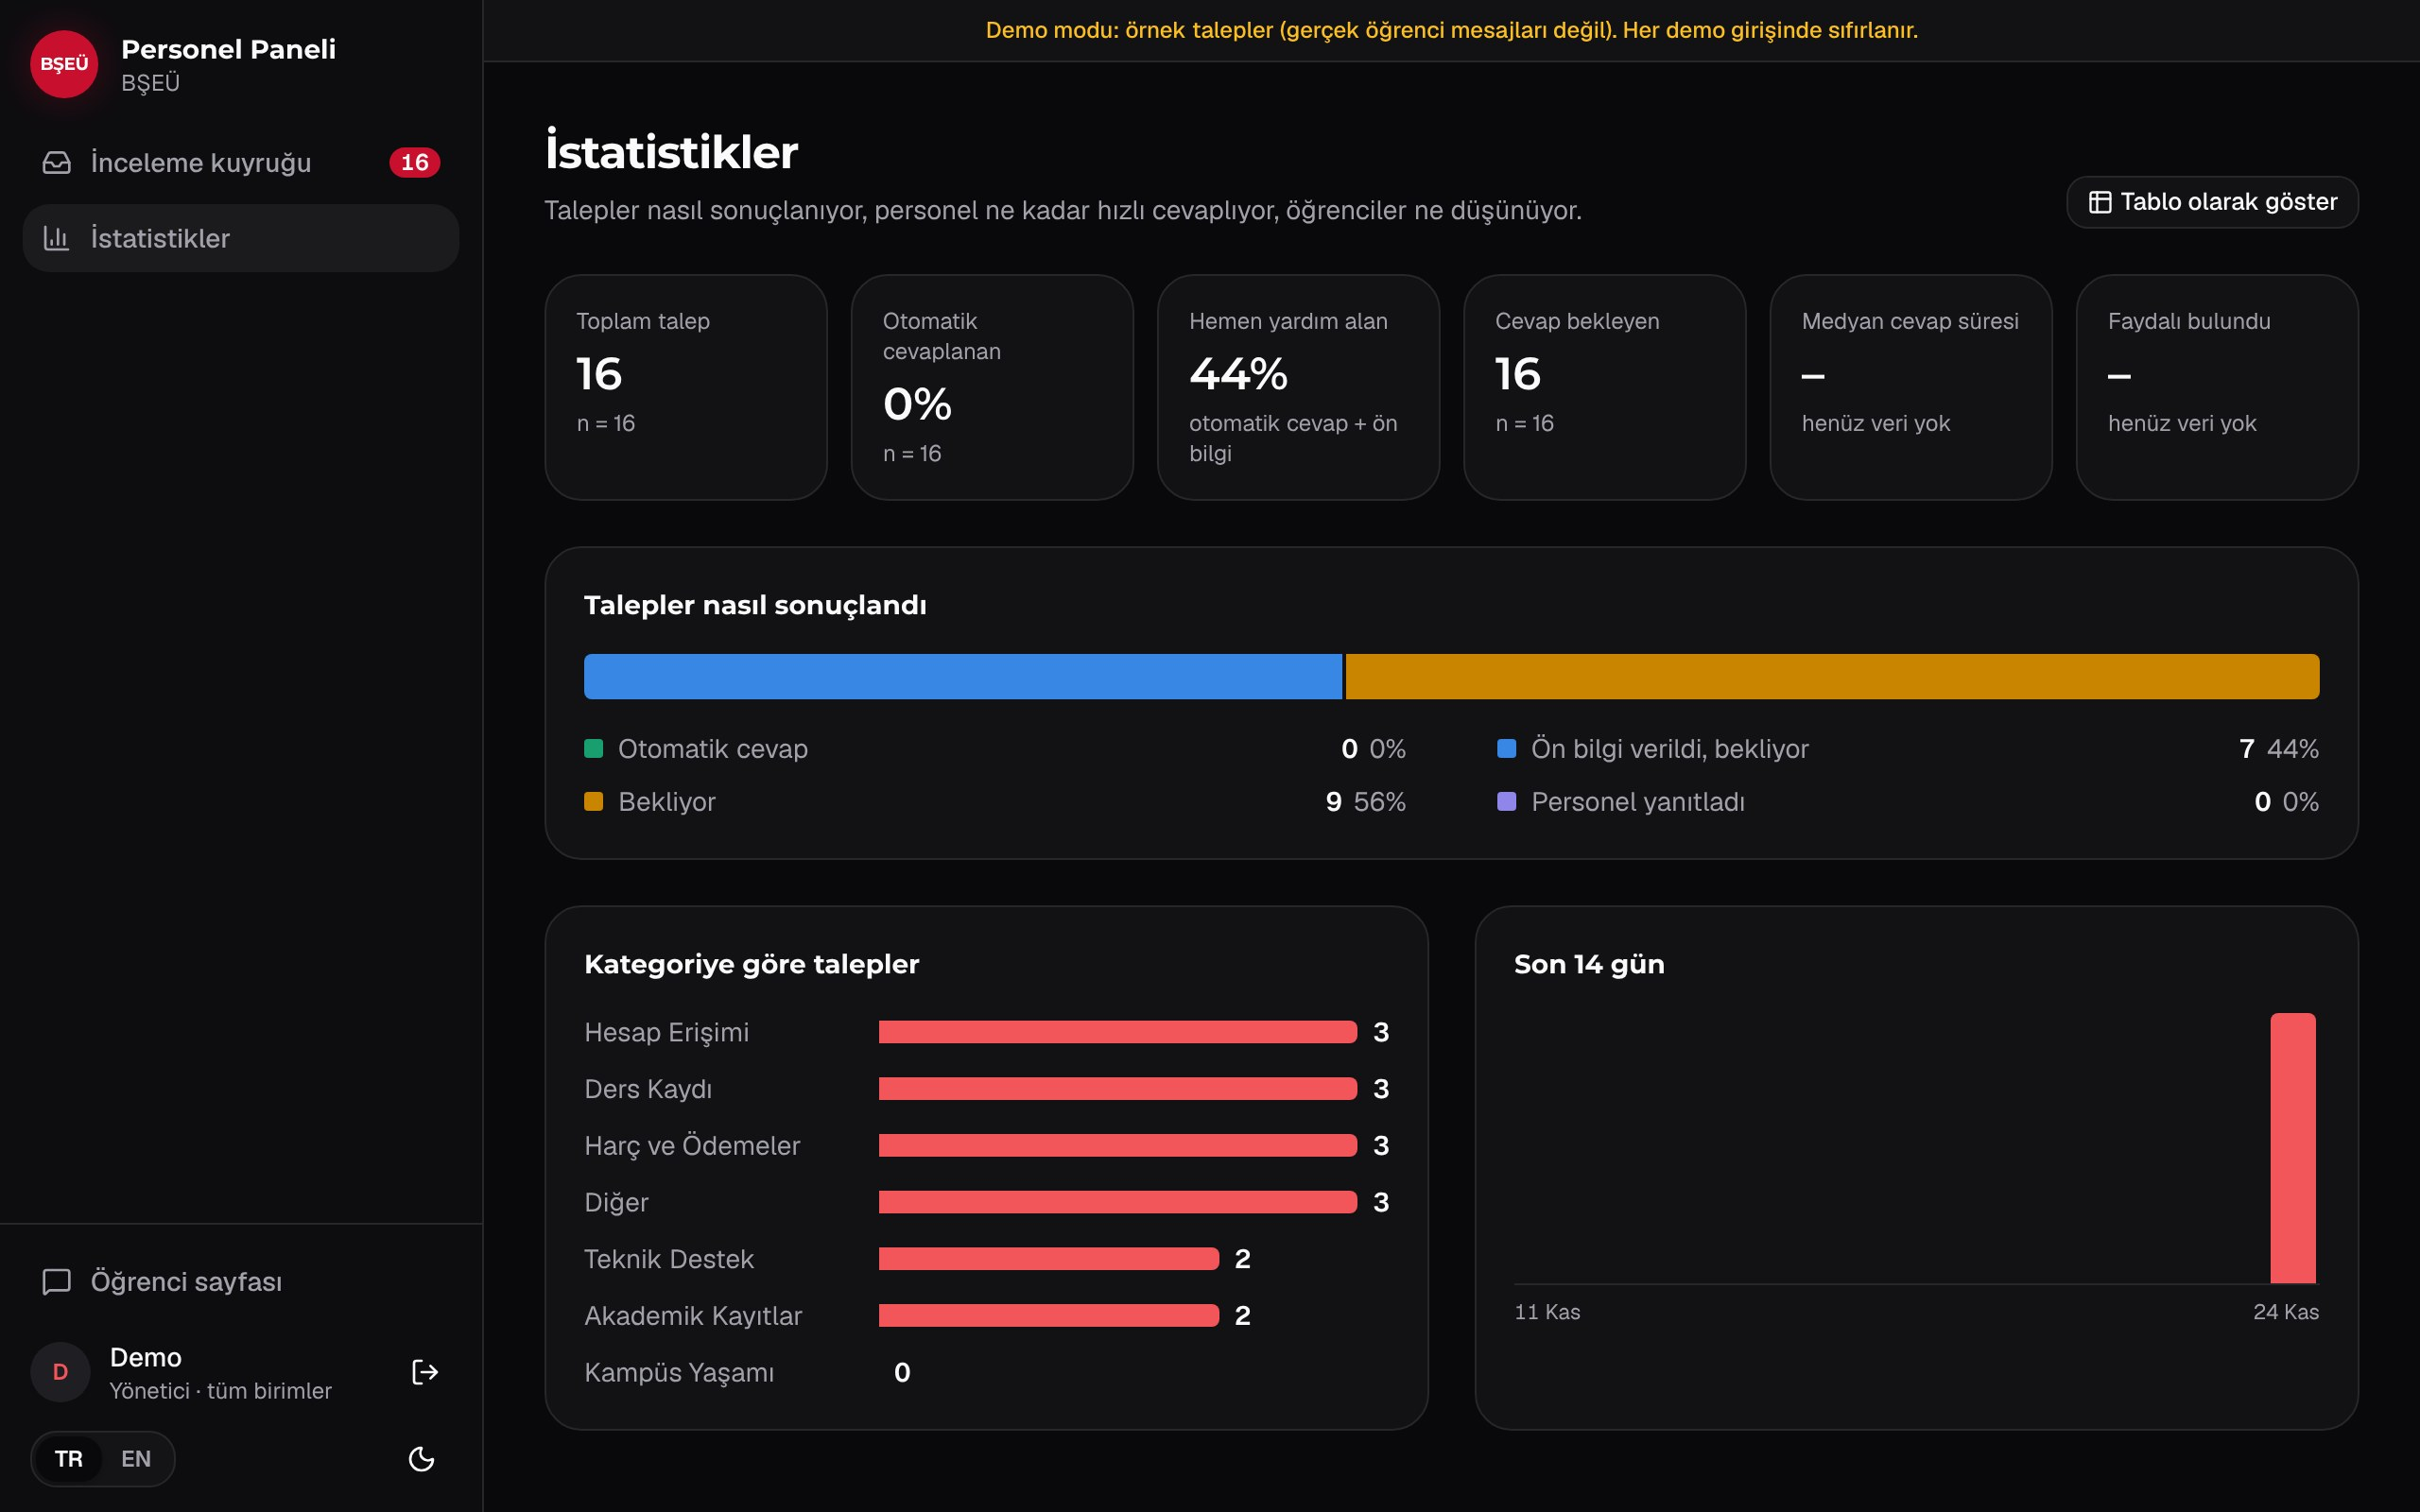
\includegraphics[width=0.95\textwidth]{sekiller/personel_istatistik.jpg}
\caption{Personel istatistik sayfası (demo verisi)}
\label{fig:istatistik}
\end{figure}

\section{Güvenlik ve Gizlilik}

Tablo~\ref{tab:guvenlik} ele alınan tehditleri ve önlemlerini özetler. Öğrencinin metni modele
gönderilmeden önce \texttt{<ticket>} etiketleri arasına ``çitlenir'' ve istem, bu etiketlerin içindeki
metnin talimat değil veri olduğunu söyler (Kod~\ref{lst:cit}). Öğrenci çiti erken kapatmaya çalışırsa
etiket önce zararsız hâle getirilir. Bu tek başına bir garanti olmadığından alıntı denetimi ikinci
savunma hattıdır.

\begin{lstlisting}[float=!ht, language=Python, caption={Talep metninin istemde çitlenmesi (\texttt{ai/fence.py})}, label={lst:cit}]
FENCE_TAG = re.compile(r"<(\s*/?\s*ticket)", re.IGNORECASE)

def fence_ticket(text: str) -> str:
    """The ticket wrapped in <ticket> tags, with fence tags inside it made harmless."""
    return f"<ticket>\n{FENCE_TAG.sub(r'(\1', text)}\n</ticket>"
\end{lstlisting}

\begin{table}[!ht]
\centering
\caption{Tehditler ve alınan önlemler}
\label{tab:guvenlik}
\footnotesize
\renewcommand{\arraystretch}{1.2}
\begin{tabularx}{\textwidth}{@{}p{4.2cm} X@{}}
\toprule
\textbf{Tehdit} & \textbf{Önlem} \\
\midrule
Talepteki prompt injection & Talep çitlenir; alıntı belgede birebir aranır (ADR~0010) \\
Ücretli modelin kötüye kullanımı & Ziyaretçi başına dakikada 5, günde 30 talep; sistem geneli günde 300 talep; model çağrısından önce denetlenir \\
Sahte istemci IP'si & Yalnızca güvenilir proxy başlığı okunur (ADR~0007) \\
Personel hesabının ele geçirilmesi & Argon2id, hesap ve adres başına kilit, tek hata mesajı, HttpOnly + Secure + SameSite çerez \\
CSRF & Değişiklik yapan her istekte aynı kaynak denetimi \\
Birimler arası erişim & Tek erişim kuralı; başka birimin talebi ``yok'' gibi görünür \\
Loglarda kişisel veri & Yalnızca kimlik, uzunluk, kod ve hata türü loglanır; bir test bunu zorunlu tutar \\
Öğrenci talep erişimi & Bir kez gösterilen rastgele 128 bit kod; yalnızca özeti saklanır (ADR~0009) \\
Geçmişin değiştirilmesi & Yalnızca eklenen \texttt{ticket\_events}, veritabanı tetikleyicisi \\
Gizli anahtarlar & Yalnızca ortam değişkeni; git ve Docker dışında; geliştirme kancaları engeller \\
\bottomrule
\end{tabularx}
\end{table}

\section{Kalite Güvencesi ve Sürekli Entegrasyon}

Her \texttt{push} işleminde GitHub Actions, Şekil~\ref{fig:ci}'deki kontrollerin tamamını çalıştırır;
Render yalnızca CI başarılıysa yeni sürümü yayına alır. Ara rapor tarihinde arka uçta gerçek bir
PostgreSQL üzerinde çalışan \textbf{316 test} (kod kapsamı \%88) ve masaüstü ile telefonda çalışan
Playwright tarayıcı testleri bulunmaktadır. Birim testlerinde model çağrıları sahte bir sağlayıcıyla
yapılır; böylece testler ücretsizdir ve her seferinde aynı sonucu verir. Gerçek model çağrıları yalnızca
değerlendirmelerde yapılır.

\begin{figure}[!ht]
\centering
\begin{tikzpicture}[node distance=3mm and 3mm, every node/.style={font=\scriptsize}]
  \node[kutu, fill=acik] (p) {git push};
  \node[kutu, right=6mm of p, fill=s1!8, draw=s1, align=left] (py) {\textbf{Python}\\ ruff (lint + biçim)\\ mypy strict\\ pytest + Postgres\\ kapsam eşiği\\ katman testi\\ OpenAPI sapması};
  \node[kutu, right=of py, fill=s2!8, draw=s2, align=left] (fe) {\textbf{Ön yüz}\\ Biome\\ TypeScript\\ derleme\\ Playwright\\ (masaüstü + telefon)};
  \node[kutu, right=of fe, fill=s3!10, draw=s3!80!black, align=left] (dk) {\textbf{Paket}\\ Docker imajı\\ derlemesi};
  \node[kutu, right=12mm of dk, fill=bseu!8, draw=bseu] (r) {Render\\yayın};
  \node[kutu, below=6mm of fe, minimum width=40mm, dashed] (q) {CodeQL + Dependabot (haftalık)};
  \draw[ok] (p) -- (py); \draw[ok] (py) -- (fe); \draw[ok] (fe) -- (dk);
  \draw[ok] (dk) -- node[etiket, above] {yeşilse} (r);
\end{tikzpicture}
\caption{Sürekli entegrasyon ve dağıtım hattı}
\label{fig:ci}
\end{figure}

Her kural ve her hata düzeltmesi için önce başarısız olan bir test yazılır, sonra kod yazılır.
Mimari kararlar ADR olarak, her değişiklik ve ölçülen etkisi bir mühendislik günlüğünde
(\texttt{docs/dev-notes/journal.md}) kayıt altındadır. Kod parçalarından bazıları
Ekler bölümünde verilmiştir.
